\chapter{LTE}\label{lte}
Mobile communications is on to its \ac{4G} of network infrastructure with \ac{LTE}. This network infrastructure is an improvement upon \ac{UMTS}, which is a \ac{3G} network. \ac{LTE} has \ac{DL} speeds of up to 300 Mbit/s and \ac{UL} speeds of 75 Mbit/swith a varying bandwidth that ranges from 1.4 MHz to 20 MHz. The development of faster downloads speed was driven by the consumers want for better quality images, faster Internet browsing and smoother video streaming.~\cite{cox2012introduction}

\section{Network Structure}\label{network structure}
The structure of the LTE network can be broken down into 3 main parts, the \ac{UE}, the \ac{E-UTRAN} and the \ac{EPC}. The UE can simply be considered as a standard mobile phone or smartphone. The purpose of the E-UTRAN is to connect a UE to the EPC and is made up of just one component, the \ac{eNodeB} or simply put base station. Figure (place holder) shows an illustration of the E-UTRAN. An UE will only communicate with one eNodeB at any time and this eNodeB is known as the Serving eNodeB. An eNodeB proves two main functions within the network; the first is to send all the radio traffic for an UE on the DL as well as receiving any traffic sent from the UE on the UL. The second function of the eNodeB is to control low-level operations such as handovers as well as provide the signalling for such operations. Due to the eNodeB's having the added complexity of controlling operations such as handovers it moves more of the processing from the core network to the edge of the network, reducing the latency of decisions being made. Every eNodeB is connected to the EPC using the S1 interface. They can also be connected to other eNodeB's by the X2 interface. This interface is mainly used for signalling and forwarding data from a serving eNodeB to a neighbouring eNodeB during a handover.

Figure place holder for E-UTRAN image.

An illustration of an EPC can be seen in Figure (place holder). It can be seen that the EPC is made up of four main components, they are the: \ac{MME}, \ac{HSS}, \ac{P-GW} and \ac{S-GW}. 
The MME provide the high-level operations for a UE such as security and managing non-radio communication data streams as well as controlling other elements within the EPC. There are very few MME's within the LTE network, generally assigned to a certain geographical region. A UE will be assigned to a single MME known as the Serving MME. 
The HSS is a central database that holds all the information about the network subscribers such as authentication and billing information.
The P-GW is the bridge between the EPC and other packet data networks such as the Internet. The P-GW uses the SGi interface to exchange data with outside networks, such as the network operator's servers.
The S-GW function is to forward data to and from the eNodeB's to P-GW, this means that the S-GW effectively acts like a router. Much like the MME a UE will be assigned to one S-GW and there will be very few within the network as a whole.

Figure place holder for EPC image.
~\cite{cox2012introduction, 3gpp2013network}

\section{Self-Organising Network}\label{self organising network}
LTE, just like any other mobile network, needs to be managed. Due to LTE being more complex than its predecessors the managed of the network has also become more complex. The use of automation can simplify management of a network greatly. A technology that can be employed in LTE is that of a Self-Organising Network. This system provides three main functions, Self-configuration, Self-optimisation and Self-healing.~\cite{feng2008self,3gpp2011self}
\begin{itemize}
  \item \textbf{Self-configuration} allows for newly installed eNodeB to be configured automatically with the basic parameters for operation.  

  \item \textbf{Self-optimisation} is a process where measurements from the UE and eNodeB along with performance measurements are used to optimise the network to make it perform better.

  \item \textbf{Self-healing} is designed to detect and identify failures within the network. After the self-healing system detects a failure it aims to recover from the failure without the need for human interaction with the system.
\end{itemize}

\section{Handover}\label{handover}
The process of handover is very important in mobile telecommunications. It involves moving the resource allocation for a mobile phone or a piece of \ac{UE} from one base station to another. This process is used to provide more \ac{QoS} to customers by allowing them to continue to use provided services even after moving out of range of the original serving base station. To keep with the QoS it is important that handovers are done fast, have little-to-no disruption to the users experience and are completed with a very high success rate. If a handover is unsuccessful it is likely that an on going call will be dropped due to there not being enough resources available on a base station, known as an \ac{eNodeB} in \ac{LTE}, or the received signal strength to the \ac{UE} drops below a certain threshold needed to maintain the call. Handovers are stated to take roughly 0.25 seconds to complete after the decision has been made for a handover to take place~\cite{jansen2010handover}.

\subsection{Parameters}\label{parameters}
In LTE there are two main parameters that are used in the handover process. These parameters are the \ac{TTT} and \ac{hys}. The hys is used to define how much better the \ac{RSS} of a neighbouring base station must be than the serving base station for a handover to be considered. The values of hys are defined in \ac{dB} and range from 0 to 10 dB in 0.5 dB increments, this results in there being 20 different values of hys. The full range of hys values can be seen in Table~\ref{tab:hys}.

\begin{table}[H]
  \begin{center}
    \begin{tabular}{| l | p{2cm} |}
  	  \hline
      Parameter & Value(dB) \\ \hline
      hys & 0.0 \newline
	  0.5 \newline
	  1.0 \newline
	  1.5 \newline
	  2.0 \newline
	  2.5 \newline
	  3.0 \newline
	  3.5 \newline
	  4.0 \newline
	  4.5 \newline
	  5.0 \newline
	  5.5 \newline
	  6.0 \newline
	  6.5 \newline
	  7.0 \newline
	  7.5 \newline
	  8.0 \newline
	  8.5 \newline
	  9.0 \newline
	  9.5 \newline	  	  	  	  
	  10.0 \\
      \hline
  	\end{tabular}
  \end{center}
  \caption{Table of the different LTE hys values.}
  \label{tab:hys}
\end{table}

The TTT is a length of time, defined in seconds, that is used to define how long a neighbouring base station must look better than the serving base station for. There are 15 different values of TTT ranging from 0 to 5.12 seconds. Unlike with hys the TTT values do not increment linearly, instead they increment exponential with smaller increases at the lower values ad bigger increases at the larger values. The full list of TTT values can be seen in Table~\ref{tab:ttt} and a graph of how the TTT values increase can be seen in Figure~\ref{fig:ttt}.

\begin{table}[H]
  \begin{center}
    \begin{tabular}{| l | p{1.5cm} |}
  	  \hline
      Parameter & Value(s) \\ \hline
      TTT & 0.0 \newline
      0.04 \newline
	  0.064 \newline
	  0.08 \newline
	  0.1 \newline
	  0.128 \newline
	  0.16 \newline
	  0.256 \newline
	  0.32 \newline
	  0.48 \newline
	  0.512 \newline
	  0.64 \newline
	  1.024 \newline
	  1.280 \newline
	  2.56 \newline
	  5.12 \\
      \hline
  	\end{tabular}
  \end{center}
  \caption{Table of the different LTE TTT values.}
  \label{tab:ttt}
\end{table}

\begin{figure}[H]
  \begin{center}
    	  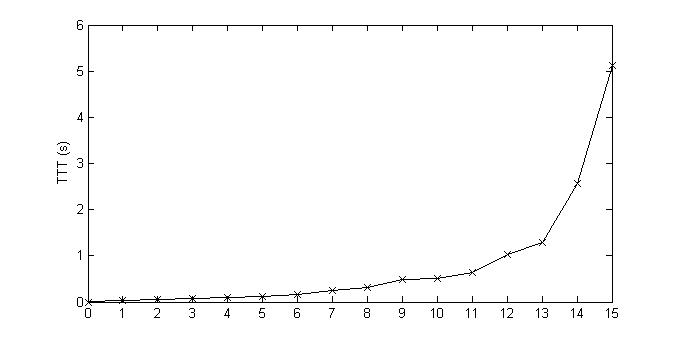
\includegraphics[width=0.5\textwidth]{figures/TTTgraph.jpg}
    \end{center}
    \caption{Graph of TTT values.}
    \label{fig:ttt}
\end{figure}

There are 336 different combinations of TTT and hys values. Having such a large range of combinations means that pairs of values can mean that a neighbouring eNodeB has to be better by a large hys but for a small TTT or vice-versa. This makes for an interesting dynamic for which pairs of values will work the best in any given environment.

\subsection{Procedure}\label{procedure}
In LTE there are eight different triggers defined for initiating handovers within LTE. Table~\ref{tab:trigger} shows different trigger events and how they are defined~\cite{3gpp2012triggers}. 

\begin{table}[H]
  \begin{center}
    \begin{tabular}{| l | p{11.1cm} |}
  	  \hline
      Event Type & Trigger Criteria \\ \hline
      A1 & Serving becomes better than a threshold. \\
      A2 & Serving becomes worse than a threshold. \\
      A3 & Neighbour becomes offset better than \ac{PCell}. \\
      A4 & Neighbour becomes better than threshold. \\
      A5 & \ac{PCell} becomes worse than threshold1 and neighbour becomes better than threshold2. \\
      A6 & Neighbour becomes offset better than \ac{SCell}. \\
      B1 & Inter RAT neighbour becomes better than threshold. \\
      B2 & \ac{PCell} becomes worse than threshold1 and inter RAT neighbour becomes better than threshold2. \\
      \hline
  	\end{tabular}
  \end{center}
  \caption{Table of the different LTE Trigger types and their criteria.}
  \label{tab:trigger}
\end{table}

Out of the eight triggers the A3 event is the most common and it is defined that a neighbouring eNodeB must give the UE better Received Signal Strength (RSS) by an amount defined by the hys, for a length of time defined by the TTT.  An illustration of how the signals from the serving and neighbouring eNodeB’s look in an A3 event can be seen in Figure (place holder). The A3 event can also be represented by the following equation:

\begin{equation}
RSS_{Neighbouring} + hys > RSS_{Serving}
\end{equation}
 
Place holder for image of event A3

When a handover event is triggered a measurement report is sent from the UE to the serving eNodeB. The measurement report contains the information required for the serving eNodeB to make a decision on whether to initiate the handover or not. If the handover is triggered the serving eNodeB will signal to the neighbouring eNodeB that is to become the new serving eNodeB. If the serving eNodeB decides not to initiate the handover then no more action is taken until another handover event is triggered.

The full, high-level, procedure for a LTE handover is as follows:
\begin{enumerate}
	\item If a neighbouring eNodeB is found to be better than the serving eNodeB a measurement report is sent by the UE to the serving eNodeB.
	\item The serving eNodeB considers the information in the measurement report and decides whether or not a handover should take place.
	\item If it is decided that a handover should take place then a message is sent to the neighbouring eNodeB to prepare resources for the UE.
	\item Once the resources are ready for the UE the new serving eNodeB sends a message to the old eNodeB to release the resources it previously had for the UE
	\item Finally a message is sent to the MME to finalise the handover process.
\end{enumerate}
